\ofsubsection{Caos em Cornelia}
%
\ofquote{"Eu, Garland derrotarei a todos vocês!"\\}{Garland}\\\\
%
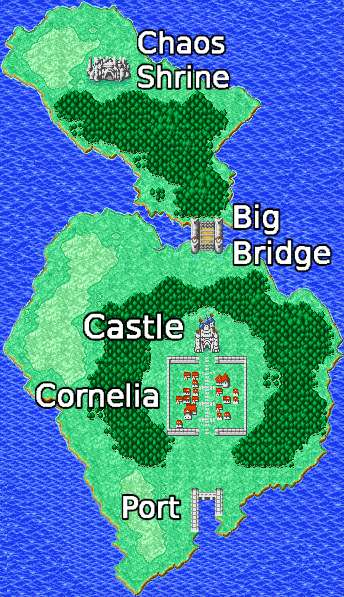
\includegraphics[width=\columnwidth]{./art/chaosincornelia/map.jpg} \ofpar
%
\accf{Caos em  Cornelia} é uma aventura preparada que se encaixa bem com jogadores e MJs inexperientes. 
Nesta aventura o grupo é incumbido de encontrar a princesa Sarah do reino de Cornelia, uma trama baseada no início do primeiro jogo de Final Fantasy.
Um mapa com todos os locais de interesse são mostrados acima, os jogadores devem criar um personagem de nível 1 de acordo com as regras de criação de personagem. 
Como a aventura começa em um navio para Cornelia, a história deles deve explicar o porquê de partirem nesta jornada.
%
\ofpar
%
\ofquote{"A lua está cansada de esperar por você!"!"\\}{Cid}\\\\
%
O grupo está em um pequeno navio de transporte chamado \accf{Bronquitito}, que está transportando carga para Cornelia.
O capitão Cid concordou em deixar o grupo embarcar por uma pequena taxa e além deles, há somente 2 outros marinheiros, Biggs e Wedge, que estão usando bandanas curtas e brancas e camisas vermelhas listradas.
Ambos são jovens e inexperientes, mas amigáveis com o grupo. Diferente do capitão que se recolhe à sua cabine, por preferir ficar sozinho.
%
\ofpar
%
\ofquote{"Eu não pareço, mas sou um covarde por dentro."\\}{Wedge}\\\\
%
Se os aventureiros não se conhecerem, eles podem se apresentar a cada um e após isso terão a liberdade de explorar o navio.
Também podem conversar com os marinheiros, que sempre ficam contentes em matar o tempo durante a viagem. 
Biggs e Wedge contam a eles sobre os recentes ataques de piratas, que parecem ter aumentado recentemente.
Além disso, também contam sobre Cornelia e como ouviram sobre o desaparecimento da princesa.
Se perguntarem sobre Cid, contarão sobre seu passado como um soldado aposentado.
À medida que escurece, a tripulação se recolhe às cabines.
Quando os aventureiros se preparam para terminar o dia, de repente ouvem barulhos ao redor do navio.
Rapidamente notam que vários piratas embarcaram no Bronquitito!
Na batalha a seguir, o grupo inimigo deve consistir de aproximadamente um pirata por jogador e dado o espaço restrito, assuma que todos estão ao alcance do outro.
Nesse meio tempo, a tripulação não está no local, pois estão lutando contra outros piratas que adentraram a parte interna do deque.
Ao derrotar os piratas, lembre de recompensar o grupo com o Gil deixado por cada inimigo.
%
\vfill
%
\ofmonster{Pirata}{1}{
\includegraphics[width=0.2\columnwidth]{./art/chaosincornelia/pirate.jpg}}
{
	PV: & \hfill 10 & PM: & \hfill 0\\
	FOR: & \hfill 1 & DEF: & \hfill 0 \\
	MAG: & \hfill 0 & RES: & \hfill 0 \\
	AGI: & \hfill 3 & Tamanho: & \hfill M\\
}
{\accf{Cimitarra}: 1d Dano \hfill \accf{Deixa:} 150G}
{}
%
\vfill
%
Após a batalha, todos se juntam e Cid agradece pela ajuda.
Ele explica que essa não é a primeira vez que eles são abordados por esses piratas, os quais fazem parte da tripulação do capitão Bikke.
Agora o grupo pode dormir para recuperar PV e PM. Logo após acordarem pela manhã, o navio aporta em Cornelia.
Uma vez lá, a tripulação começa a descarregar as mercadorias e se despede do grupo.
O porto de Conelia é pequeno e comporta somente poucos navios de carga semelhantes ao Bronquitito.
Os marinheiros no porto descarregam caixas dos navios, tanto para armazená-los nos galpões quanto diretamente a Cornelia.
%
\vfill
%
\ofquote{"A propósito, precisa de algo? Pode dar uma olhada nos meus produtos! Você pode se surpreender com o que vai encontrar."\\}{Dyce}
%
\clearpage
%
Depois de desembarcar do navio, o grupo pode perguntar pelo caminho até Cornelia.
Os marinheiros os avisam para terem cuidado no trajeto, pois os guardas do castelo não estão mais patrulhando a rota.
Cornelia não é muito distante do porto e o caminho leva através dos campos e campinas na maioria das vezes.
O grupo pode se encontrar com um mercador viajante chamado \accf{Dyce} no porto.
Ele é um homem atlético, alto, careca, tem barba e traja vestes pretas.
Também tem uma Chocobo na qual viaja.
Dyce fornece ao grupo, a informação sobre os problemas em Cornelia, pois ouviu rumores de que a princesa foi raptada.
Também vende poções por 125G cada, mas possui mais coisas as quais o grupo não pode pagar por enquanto.
Dyce é um viajante, então é provável que cruzem com ele novamente no futuro.
No entanto, seus preços são normalmente acima das lojas comuns.
%
\ofpar
%
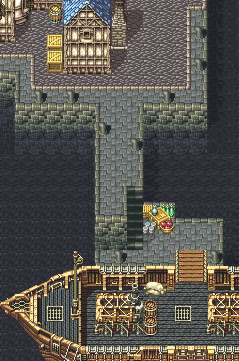
\includegraphics[width=\columnwidth]{./art/chaosincornelia/port.jpg} \ofpar
%
\ofquote{"Você deve ter culhões de aço para me desafiar!"}{Bikke}\\\\
%
Ao falar com Dyce ou outros marinheiros, o grupo descobre que o porto é atacado por piratas com frequência.
Geralmente, a área é protegida pelos guardas de Cornelia, mas desde o desaparecimento da princesa, o rei convocou todas as tropas ao castelo. 
Os piratas sempre atacam à noite e se o grupo ficar por um tempo no porto, testemunharão esses ataques noturnos.
Assim que o grupo conhecer os planos dos piratas, eles podem tentar tomar medidas defensivas como armar uma emboscada ou armadilhas de antemão.
Os ataques começam com um grande navio pirata aportando nas docas e vários piratas invadindo para pilhar os galpões e outros navios.
Eles são, mais uma vez, a tripulação do capitão Bikke, mas desta vez o próprio se encontra presente.
Na luta a seguir, Bikke permanece recuado e bate em retirada ao seu navio se receber algum dano.
Há também alguns de seus homens ao seu lado, novamente, aproximadamente um pirata por jogador.
Como é provável que Bikke fugirá da batalha, o grupo pode se encontrar com ele futuramente.
Após rechaçar os piratas com sucesso, os marinheiros no porto estarão muito agradecidos e oferecerão comida e acomodações de graça pela noite.
%
\vfill
%
\ofmonster{Bikke}{2}{
\includegraphics[width=0.2\columnwidth]{./art/chaosincornelia/pirate2.jpg}}
{
	PV: & \hfill 32 & PM: & \hfill 25\\
	FOR: & \hfill 1 & DEF: & \hfill 2 \\
	MAG: & \hfill 1 & RES: & \hfill 2 \\
	AGI: & \hfill 2 & Tamanho: & \hfill M\\
}
{\accf{Cimitarra}: 1d Dano}
{	
	\mspell{Raio}{4}{0r}{Único}{3u}{CAuse 2d de dano de Raio ao alvo.}{\lightning}	
	\mtech{Animar}{5}{0r}{Único}{3u}{O alvo ganha AuFOR por 1 rodada.}{\enstr}	
}
%
\vfill
%
Abaixo está o mapa de \accf{Cornelia}, há também algumas fazendas ao redor da cidade que não são mostradas.
Todos os locais de interesse estão marcados com números e a seguir, você pode encontrar parágrafos com tais números dando detalhes sobre cada local.
O grupo chega a Cornelia pelo portão sul, onde dois guardas os param por não os conhecer. 
Eles os aconselham a ficar longe do castelo e deixar a cidade após terminarem o que quer que tenham vindo fazer.
A maioria dos cidadãos estão muito assustados para deixar suas casas desde que a princesa desapareceu.
%
\ofpar
%
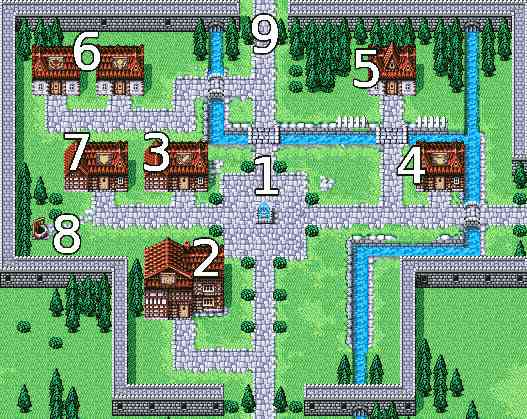
\includegraphics[width=\columnwidth]{./art/chaosincornelia/cornelia.jpg}
%
\clearpage
%
\ofquote{"Olá! Eu sou uma dançarina! O que é isto? Gosta de dança? Hee hee!"}{Arylon}\\\\
%
\accf{1. Fonte:} O grupo nota uma linda fonte que se destaca na, antes impressionante, cidade. 
Próximo a ela há uma jovem de cabelos azuis, muito animada, usando um vestido vermelho, praticando sua dança, seu nome é Arylon.
Ao ser questionada sobre a princesa ou sobre o castelo, ela conta rumores de que a princesa Sarah está sendo mantida como refém em troca de um grande resgate.
Portanto, o castelo está um caos e foi trancado.
Ela também revela que já houve várias tentativas de resgatar a princesa.
%
\vfill
%
\ofquote{"Por favor, entre! Cobramos 50G o pernoite. Gostaria de ficar?"}{Elia}\\\\
%
\accf{2. Pousada:} O grupo entra numa pequena sala com um tapete vermelho no piso e um balcão no canto.
Atrás do balcão está uma jovem com cabelos azul escuros, usando um longo vestido verde, seu nome é Elia.
À esquerda, está um grande quarto com várias camas e pequenas decorações nas paredes onde os hospedes repousam.
À direita, outro quarto com cadeiras de madeira e mesas para os hospedes sentar, comer e beberem.
O grupo pode dormir na Pousada por 50G a noite por pessoa.
Eles também podem pedir a Elia por informações, pois ela acaba ouvindo bastante dos visitantes.
Ela informa sobre várias pessoas na cidade de quem o grupo pode se interessar, como o ferreiro e os magos.
%
\vfill
%
\accf{3. Ferreiro:} O grupo entra numa loja grande com uma forja.
Atrás do balcão está um velho com cabelos castanhos e uma barba cheia, seu nome é Todo.
Ele informa que a loja está fechada e que não pode trabalhar devido a não estar recebendo as remessas necessárias do porto. 
Para ajudá-lo, o grupo pode falar com Dyce no porto de Cornelia, que está tratando das remessas.
Eles consistem em grandes caixas de madeira numa pequena carroça, a qual diminui o movimento do carregador.
No caminho de volta à Cornleia, um monstro bizarro chamado \accf{PuPu} tenta roubar as remessas!
A criatura está sentada nas árvores e usa sua habilidade de \accf{Abduzir} para fazer a caixa desaparecer.
Se os jogadores procurarem por ele nas árvores enquanto faz isso, ele é achado com facilidade, porque o topo de sua cabeça está brilhando.
Do contrário, ele é difícil de encontrar, um jogador deve fazer um teste de DC entre 6-8.
O grupo pode falhar em encontrar o PuPu, mas ele estará nos arredores se retornarem depois. Se detectado, PuPu não luta, ao invés disso ele usa \accf{Poções,~Por favor!} e devolve os produtos roubados se o grupo concordar.
Eles também podem apenas atacá-lo, neste caso a remessa reaparece depois dele ser derrotado.
Se retornarem a carga com sucesso, Todo recompensará o grupo com 500G.
O ferreiro pode trabalhar novamente, mas ele estará ocupado por algum tempo, finalizando encomendas.
Quando o grupo retornar em alguns dias, Todo pode vender-lhes armas e armaduras de nível Iniciante.
%
\newpage
%
\ofmonster{PuPu}{?}{
\includegraphics[width=0.15\columnwidth]{./art/chaosincornelia/pupu.jpg}}
{
	PV: & \hfill 10 & PM: & \hfill 10\\
	FOR: & \hfill 0 & DEF: & \hfill 0 \\
	MAG: & \hfill 0 & RES: & \hfill 0 \\
	AGI: & \hfill 2 & Tamanho: & \hfill P\\
}
{\accf{Deixa}: Tudo roubado{}}
{	
	\mtech{Abduzir}{0}{1r}{Único}{5u}{
		Um objeto que você pode ver ao alcance, desaparece para um local desconhecido.
	}{}	
	\mpassive{Poções por favor!}{
		Peça a seus inimigos para lhe darem uma Poção, se eles concordarem faça um teste de DC 7. 
		Se bem sucedido, desapareca para um local desconhecido (KO), do contrário, continue pedindo por mais.
	}
}
%
\vfill
%
\accf{4. Loja:} Este armazém geral é dominado por um grande balcão no centro e montes de mercadorias e itens ao redor.
Atrás do balcão está um jovem de cabelos escuros, usando uma bandana verde, seu nome é Guston.
Ele não está tão preocupado com a princesa, mas está aborrecido porque esse problema na cidade atrapalhou seus negócios.
Portanto, ele é bem amigável com clientes em potencial e vende os seguintes itens.
%
\ofpar
%
\oftable
{p{0.14\columnwidth} p{0.14\columnwidth} l} 
{\accf{Item} & \accf{Preço} & \accf{Efeito}}
{	
	Grama eco 		& 50G & Remove Mudo.  \ofrow
	Poção    		& 100G & Recupera 8 PV. \ofrow
	Etér 			& 150G & O alvo recupera 12 PM.\ofrow
	Pena da Fênix	& 300G & Remove KO e recupera 1 PV. \ofrow
	Tenda 			& 500G & Permite ao grupo dormir no ermo. \ofrow
	Lanterna 		& 100G & Ilumina uma área até 10u.
}
%
\vfill
%
\ofquote{"Não desanimem, bravos guerreiros."\\}{Gregory}\\\\
%
\accf{5. Capela:} A capela é pequena e aconchegante, com bancos de madeira, mas está completamente variz exceto por uma pessoa, o padre Gregory.
Ele é um velho com uma longa barba, vestindo um robe com capuz, fala pausadamente e com calma.
Lamenta que ninguém tem visitado a capela desde o desaparecimento de Sarah.
Aparentemente, a maioria dos cidadãos acreditam que o incidente é uma punição divina, então evitam o lugar.
Gregory pede ao grupo que restaurem a fé dos cidadãos de Cornelia.
Eles podem convencer as pessoas a esclarecer os detalhes sobre o desaparecimento de Sarah (seu rapto), por exemplo.
Se eles conseguirem convencer pelo menos 3 pessoas da cidade a comparecer à capela, o padre os recompensará com 500G com satisfação.
Além disso, ele oferece seus serviços ao grupo de graça: ele pode curar KO ao realizar um longo ritual de 1h.
%
\clearpage
%
\accf{6. Os magos:} Estas duas construções são quase idênticas, cada uma consiste em uma grande sala com camas e prateleiras com montes de magias, produtos de alquimia e livros. 
Elas são habitadas por dois excêntricos e teimosos irmãos gêmeos, Gilles e Noah.
Gilles é um mago negro que veste um robe azul e um chapéu pontudo, enquanto Noah, um mago branco, veste um robe com capuz branco com adornos vermelhos.
Os outros cidadãos normalmente os evitam, exceto quando precisam de seus serviços.
Irritando-se com isso, decidiram desenvolver um frasco, o qual os permitem armazenar sua magia, dessa forma, os outros podem usá-los sem que eles estejam presentes.
Infelizmente, algo deu errado durante o desenvolvimento, fazendo com que o item quebrasse numa explosão violenta, resultando no que o grupo pode ver no quintal.
Orgulhosos, ambos culpam um ao outro pelo acidente e pararam de se conversar desde então.
O grupo pode resolver a disputa ao convencê-los de que eles são ambos culpados.
Primeiro, o grupo tem de reparar o frasco quebrado seja por meios mecânicos ou mágicos, o que for mais fácil.
Então, terão de estudar o frasco e a receita, as quais podem conseguir com os magos.
Um personagem que usa magia, logo consegue entender o problema, aqueles que não podem, terão que realizar um teste de DC 8 para saber que: O frasco quebrou porque, durante a criação, cada mago conjurou mais do que 3 magias nele, causando uma sobrecarga, pois o item suporta até 3 magias armazenadas.
Isso pode ser averiguado ao se conjurar 3 magias nele. 
Se o grupo conseguir convencer os magos, eles aceitam o erro e desculpam um ao outro.
Presenteiam o grupo com o frasco como demonstração de gratidão, assim os personagens podem visitá-los a partir de então e comprar os acessórios Iniciantes, como mostrado na tabela abaixo, embora mais possam ser adicionados.
%
\ofpar
%
\oftable
{p{0.28\columnwidth} p{0.15\columnwidth} p{0.47\columnwidth}} 
{\accf{Acessório} & \accf{Preço} & \accf{Efeito}}
{	
	Frasco mágico & 900G & Armazene até 3 magias nele. O usuário pode usa-lo com um ação para liberar o efeito das magias armazenadas no alvo.\ofrow
	Bracadeiras Rúnicas & 500G & RES +1 \ofrow
	Escudo Mithril & 500G & DEF +1
}
%
\vfill
%
\accf{7. Construção abandonada:} Esta construção foi deixada vazia de propósito, para o caso de necessidade. 
Pode ser relacionado à história do personagem ou conter algo que queira adicionar à aventura depois.
Do contrário, a casa está vazia e os jogadores podem perguntar ao redor a fim de descobrir que era usada como uma loja, abandonada por não ser lucrativa. 
%
\vfill
%
\accf{8. Poço:} É um poço. Parece possível descer por ele, mas na verdade não o faça.
%
\newpage
%
\accf{9. Entrada do Castelo}  Esta entrada leva diretamente ao \accf{Castelo de Cornelia} e está permanentemente bloqueada pelos guardas. 
Entretanto, eles deixam os aventureiros atravessar se explicarem que querem encontrar a princesa.
Os guardas pedem ao grupo para se reportarem ao chanceler no andar de cima. Um mapa dos andares do castelo, com todos os locais de interesse se encontra à direita.
A escadaria central leva ao salão do trono, enquanto a de trás, ao jardim do palácio. O qual está repleto de guardas armados o tempo todo.
%
\vfill
%
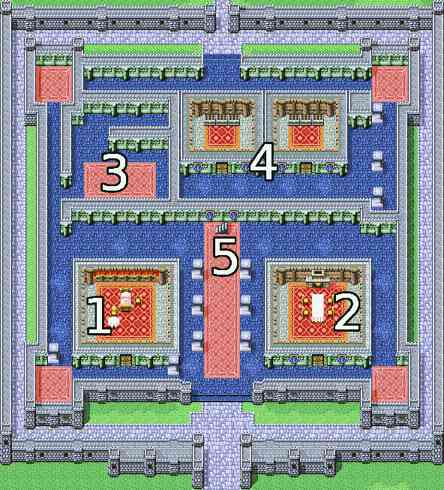
\includegraphics[width=0.96\columnwidth]{./art/chaosincornelia/castle.jpg}
%
\vfill
%
\ofquote{"Por favor, tragam-me minha filha, minha Sarah, sã e salva."}{Rainha Jayne}\\\\
%
\accf{1. Quarto da rainha:} A rainha Jayne é uma mulher de meia idade com cabelo turquesa e olhos azuis. Traja um longo vestido vermelho e uma tiara dourada. 
Ela está depressiva desde o rapto de sua filha e somente fala com o grupo depois deles terem ganhado a confiança do rei.
Assim que falar, ela lhes conta sobre a noite do rapto, cujo qual testemunhou.
Uma noite, ela acordou e encontrou o Garland escapando com a princesa inconsciente em seus braços.
Ele a disse para que abdicasse do trono de Cornelia se quisesse ver sua filha viva. Então desapareceu com a garota através da entrada traseira do palácio.
A rainha está traumatizada pelo acontecido e culpa a si mesma por não poder impedi-lo.
%
\ofpar
%
\accf{2. O quarto da irmã:} Este quarto é ocupado por Alison, irmã de Sarah, uma jovem sensível que lembra sua mãe. 
Os guardas à porta dizem ao grupo que ela se trancou e não a abrirá.
Se a convencerem, garantindo que salvarão a Sarah por exemplo, ela abrirá a porta para conversar.
Alison conhece bem sua irmã, devido ao fato de se espelhar muito nela.
Ela conta ao grupo sobre a paixão de Sarah pela música e que o precioso alaúde dela desapareceu assim como sua irmã.
Se os personagens conseguirem acamá-la, eles terão uma chance melhor de também convencer o rei.
%
\clearpage
%
\ofquote{"Garland já foi um grande cavaleiro do reino. Mas o poder o corrompeu e ele se voltou contra sua própria natureza."}{Ian}\\\\
%
\accf{3. Capitão:} O capitão da guarda é um jovem com longos cabelos dourados, chamado Ian, ele veste um armadura pesada decorada e tem sua espada longa às costas.
Relutantemente, ele conversa com os aventureiros, que percebem que ele não tem o braço esquerdo.
Se o grupo já convenceu o rei, o capitão conversará com eles de boa vontade sobre a missão de resgate da princesa, a qual lidera.
Logo após o desaparecimento de Sarah, ele e seus homens seguiram Garland e o confrontaram na Grande ponte, ao norte de Cornelia.
Entretanto, Garland superou a todos na batalha que se seguiu e o capitão é o único sobrevivente.
Ele está envergonhado por seu fracasso e parece profundamente perturbado e amedrontado com o poder do vilão.
%
\ofpar
%
\accf{4. Salão do tesouro:}
Ambas as salas do tesouro são guardadas por dois homens em armaduras pesadas. Se o grupo obter uma carta do rei, eles podem receber os seguintes itens deles:
Uma grande tenda onde cabem todos eles, uma poção e 200G por membro.
%
\ofpar
%
\ofquote{"Garland não é mais o homem que conheci. Eu vos imploro. Por favor, tragam-me minha filha o mais rápido possível!"}{Rei de Cornelia}\\\\
%
\accf{5. Salão do trono:} A porta é guardada por dois guardas com glaives e armaduras pesadas. 
Do lado de dentro, o rei está sentado em seu trono e o chanceler está ao seu lado.
O rei é um homem de meia idade, de olhos azuis e cabelos castanhos, possui uma longa barba, usa uma coroa dourada e longos robes vermelhos.
O chanceler é um pouco mais jovem, com cabelos escuros e veste roupas nobres.
O rei está feliz em ver os aventureiros, por estar desesperado para encontrar sua filha, mas o chanceler está cético.
Na conversa a seguir, o grupo pode tentar convencer o rei de que eles podem resgatar a Sarah, mas o chanceler o convence de que devem provar seu valor primeiro.
O rei lamenta que tenha negligenciado seu povo enquanto tem tentado resgatar sua filha.
Ele pede ao grupo para ajudar o povo de Cornelia e provar que são capazes de salvar a princesa. Em retribuição, promete fornecer os suprimentos para a viagem.
Ao completar algumas das seguintes tarefas, o rei pode ser convencido: ajudar o ferreiro a receber as remessas, resolver a disputa entre os dois magos, defender o porto dos piratas e ajudar a capela a recuperar seus fiéis.
Após ganhar a confiança do rei, ele revela mais detalhes do rapto: Sarah foi sequestrada por um antigo cavaleiro de Cornelia, chamado Garland, o mais poderoso espadachim do reino.
Ele costumava ser próximo ao rei, mas o poder o corrompeu e ele exigiu ser seu sucessor.
Quando o rei negou, Garland raptou sua filha como refém pelo controle do reino.
Muitos outros cavaleiros tentaram salvá-la, mas nenhum foi bem sucedido. Descobriram que a princesa é mantida no Santuário do caos, ao norte de Cornelia, além da Grande ponte.
O rei mantém sua promessa e escreve uma carta para confirmar que ao grupo foi dada a missão de resgatar sua filha.
Esta carta os permite conseguir suprimentos da tesouraria e os outros membros do palácio se mostrarão dispostos a conversar com eles.
Após convencer o rei com sucesso, o grupo é recompensado com um \accf{Nível} a mais!
%
\vfill
%
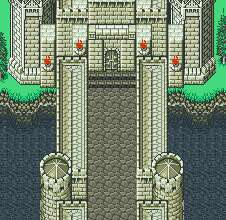
\includegraphics[width=\columnwidth]{./art/chaosincornelia/bridge.jpg} 
%
\vfill
%
\ofquote{"Vamos ver como vocês lidam com o poderoso Eu! E ao dizer eu, quero dizer Gilgamesh!! E ao dizer lidam, quero dizer MORREM!"}{Gilgamesh}\\\\
%
Ao partir de Cornelia e se encaminhar ao norte, o grupo se encontra nas florestas e campinas circundantes ao castelo.
Após várias horas de viagem através da calma natureza, eles chegam à Grande ponte, que é tão massiva quanto velha e frágil.
Ao chegarem ao fim dela, encontram Gilgamesh, que parece os estar esperando.
Ele não é necessariamente bom ou mal, apenas viaja o mundo em busca de poderosas armas para sua coleção.
Garland o convenceu a trabalhar para ele, em retorno a ele seria presenteada a lendária espada "Excalibur".
Ao encontrar o grupo, Gilgamesh os reconhecem como potenciais oponentes valorosos e saca sua espada, seu modo de combate é detalhado abaixo.
Ao ser reduzido a 0 PV, ele não desmaia de imediato, ao invés disso, finalmente saca a Excalibur para um último golpe.
Ao tentar fazer isso, a espada não causa dano e se quebra no mesmo momento. Gilgamesh percebe que foi enganado e sem ver outra opção, foge.
Por continuar vivo, o grupo pode encontrá-lo futuramente.
O grupo então pode finalmente cruzar a ponte e chegar à floresta das trevas antes do Santuário do caos.
A floresta é estranhamente quieta e a maioria de suas árvores e plantas parecem ter morrido.
É bem possível que os aventureiros não cheguem ao Santuário antes do anoitecer, então eles devem passar a noite aqui.
%
\clearpage
%
\ofmonster{Gilgamesh}{2}{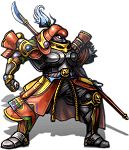
\includegraphics[width=0.2\columnwidth]{./art/chaosincornelia/gilgamesh.jpg}}
{
	PV: & \hfill 45 & PM: & \hfill 40\\
	FOR: & \hfill 2 & DEF: & \hfill 1 \\
	MAG: & \hfill 0 & RES: & \hfill 0 \\
	AGI: & \hfill 4 & Tamanho: & \hfill M\\
}
{\accf{Arma de haste}: 1d Dano \hfill \accf{Deixa}: 500G}
{	
	\mtech{Garra mortal}{6}{0r}{Único}{Arma}{
		Ataque duas vezes contra o alvo e se pelo menos um deles acertar, ele fica Imóvel por 1 rodada.
	}{\immobile}	
	\mtech{Dança de espadas}{8}{1r}{3u}{Você}{Ataque contra todos na área alvo.}{}
	\mreaction{Últimas forças}{Ao chergar abaixo de 20 PV, ganhe AuFOR até o fim da batalha.}	
}
%
\ofpar\\\\\\
%
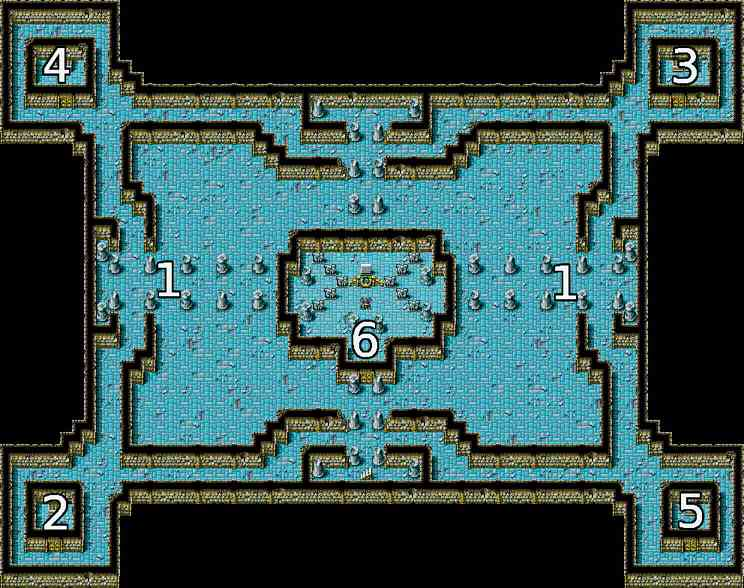
\includegraphics[width=\columnwidth]{./art/chaosincornelia/shrine.jpg} 
%
\\\\
%
À medida que o grupo alcance a borda da floresta das trevas, eles podem ver o ameaçador \accf{Santuário do caos} à distância. Ao se aproximarem, percebem que o Santuário foi tomado pela natureza, e suas paredes estão danificadas e cobertas pela vegetação, e sua fundação começou a afundar no chão.
Uma tranquilidade sobrenatural permeia o Santuário, sem qualquer forma de vida à vista, e a única entrada é um conjunto de escadarias frágeis que levam para dentro da escuridão.
Após descê-las, o grupo se encontra ao sul do mapa mostrado acima e mal podem ver devido à escuridão.
O caminho ao norte está bloqueado por destroços que é o resultado de pilares e grandes rochas que despencaram do teto.
Sob avaliação minuciosa, o grupo percebe que esse bloqueio foi propositalmente criado.
%
\newpage
%
\accf{1. Armadilhas:} Ambos os locais marcados contém uma armadilha mágica no chão que foram colocadas por Garland a fim de o alertar e impedir intrusos.
Um personagem que procure ativamente por armadilhas ou se previnam de alguma maneira, as percebem ao realizar um teste de DC~7.
A armadilha explode ao ser pisada, causando 1d+3 de dano de Fogo a todos dentro de 1u de seu centro.
%
\ofpar
%
\accf{2. Mímico:} Dentro desta sala está um grande baú, que ao ser tocado se revela ser um maligno mímico. 
Um personagem pode notar que algo está errado com o baú antecipadamente, ao realizar um teste de DC~8.
Em caso de falha, o mímico terá uma rodada surpresa no começo da batalha que se seguirá.
%
\\\\
%
\ofmonster{Mímico}{2}{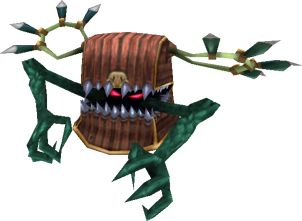
\includegraphics[width=0.28\columnwidth]{./art/chaosincornelia/mimic.jpg}}
{
	PV: & \hfill 20 & PM: & \hfill 0\\
	FOR: & \hfill 2 & DEF: & \hfill 0 \\
	MAG: & \hfill 0 & RES: & \hfill 0 \\
	AGI: & \hfill 2 & Tamanho: & \hfill M\\
}
{\accf{Mordida}: 1d Dano \hfill \accf{Deixa} 200G}
{}
%
\ofpar
%
\accf{3. Fonte de cura:} A porta pesada desta sala está trancada e pode ser quebrada ou arrombada, com um teste bem sucedido de DC entre 6 e 9, a depender da habilidade do personagem. 
Dentro da sala, o grupo encontra um grande cálice, que jaz num pedestal de pedra e está cheio com o que se parece água.
Após inspeção minuciosa, um personagem pode entender que o líquido é de natureza mágica e que pode ser bebido, recuperando PV e PM completamente.
Entretanto, o cálice em si não possui propriedades mágicas e contém apenas 5 porções de sua água curativa.
%
\ofpar
%
\accf{4. Baús:} Esta sala contém 2 baús, um deles pode ser aberto com facilidade e contém 3 poções e uma pena de fênix. 
O outro, \accf{O alaúde de Sarah} e pode somente ser arrombado ao realizar um teste de DC que vai de 7 a 10, a depender da habilidade do personagem.
Também é possível abrir com a chave que Garland carrega consigo, mas o baú é muito robusto para ser quebrado à força.
%
\ofpar
%
\accf{5. Porta secreta:} Esta sala está vazia exceto pela grande tabula à parede à esquerda, que possui vários símbolos nela. 
Sob inspeção minuciosa, o grupo pode entender que os símbolos descrevem uma curta música.
A parede próxima contém uma porta secreta a qual é revelada ao se tocar a música no alaúde de Sarah, embora somente ela seja capaz de executá-la apropriadamente.
A porta secreta leva até uma pequena sala com um pedestal de pedra sobre o qual jaz um anel dourado.
O acessório Iniciante é chamado de \accf{Anel angelical} e tem o seguinte efeito: ao sofrer KO enquanto o usando, você pode ativar seu efeito de imediato, revivendo com 1 PV. O anel é então destruído.
%
\clearpage
%
\ofquote{"Humf. Os cachorrinhos do rei. Sabem com quem estão mexendo?"}{Garland}\\\\
%
\accf{6. Garland:} No centro do templo, o grupo finalmente confronta o Garland. 
Sarah também se encontra aqui, enjaulada no canto. Garland é alto, atlético, usa uma armadura pesada, veste uma capa púrpura e carrega sua espada.
É muito arrogante e acredita que merece comandar Cornelia, porque ele é o guerreiro mais forte do reino.
Ele estuda as artes das trevas do Santuário do caos desde sua chegada a fim de expandir seu poder.
Garland vê o grupo apenas como mais uma pedra no caminho de seus grandes planos.
%
\vfill
%
\ofquote{"Você realmente acha que tem o necessário para cruzar espadas COMIGO? Veremos..."}{Garland}\\\\
%
Garland saca sua arma e começa a luta, além de invocar vários morcegos em seu auxílio, um para cada membro do grupo.
Durante a batalha, ele foca em se posicionar a fim de mirar em membros solitários, enquanto evita ser superado em números.
Na história original, Garland usa um artefato mágico para escapar depois de ser derrotado e se torna o antagonista principal do jogo.
Se quiser continuar a aventura de maneira diferente, ele também pode morrer na mão dos aventureiros ou deixe que os próprios decidam o destino dele.
Após ser libertada da prisão, Sarah está paralisada, muito assustada e traumatizada.
Ela agradece ao grupo por resgatá-la e pede que encontrem seu precioso alaúde. 
O grupo pode recusar o pedido e logo retornar para Cornelia. Sarah entenderá, mas não ficará feliz.
%
\vfill
%
\ofmonster
{Garland}{3}{
\includegraphics[width=0.2\columnwidth]{./art/chaosincornelia/garland.jpg}}
{
	PV: & \hfill 40 & PM: & \hfill 50\\
	FOR: & \hfill 3 & DEF: & \hfill 2 \\
	MAG: & \hfill 2 & RES: & \hfill 1 \\
	AGI: & \hfill 2 & Tamanho: & \hfill M\\
}
{\accf{Espada longa}: 1d Dano \\ \accf{Deixa}: 1000G, Chave \\ \accf{Auto-Oscilar, Golpe duplo}}
{
	\mspell{Fogo}{4}{0r}{Único}{3u}{O alvo sofre 2d de dano de Fogo.}{}	
	\mspell{Drenar}{6}{0r}{Único}{4u}{Reduza o PV do alvo em 1d e regenere o seu PM na mesma quantidade.}{}	
	\mspell{Silenciar}{6}{0r}{Único}{5u}{O alvo faz um teste de DC 8 ou fica Mudo por 3 rodadas.}{\silence}
}
%
\newpage
%
\ofmonster
{Morcego}{1}{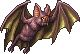
\includegraphics[width=0.2\columnwidth]{./art/chaosincornelia/bat.jpg}}
{
	PV: & \hfill 6 & PM: & \hfill 0\\
	FOR: & \hfill 0 & DEF: & \hfill 0 \\
	MAG: & \hfill 0 & RES: & \hfill 2 \\
	AGI: & \hfill 4 & Tamanho: & \hfill P\\
}
{\accf{Presas}: 1d Dano \\ \accf{Deixa:} 100G }
{\mpassive{Absorver}{Cada ataque bem sucedido recupera 1d PV.}}
%
\vfill
%
\ofquote{"Vocês...Vieram me resgatar? Jamais saberei como agradecer..."}{Sarah}\\\\
%
Após resgatar a princesa, o grupo pode levá-la para Cornelia em segurança e, portanto, terão que viajar de volta.
A jornada deve ser calma, mas você pode adicionar algumas surpresas se quiser.
Sarah é uma jovem princesa de cabelos turquesa como os da mãe, traja um vestido tingido de dourado e um pendente de joias vermelhas.
Ele é educada, mas também muito quieta e avoada, pois está sofrendo física e mentalmente das cicatrizes de seu rapto.
Ela não é capaz de cuidar de si mesma, precisando que os aventureiros a guiem durante a jornada. Enquanto viajando, com frequência pergunta sobre o estado do reino e de sua família, pois se culpa pelo acontecido.
%
\vfill
%
\ofquote{"Obrigado por trazerem minha filhar de volta ao meu lado." \\}{Rei de Cornelia}\\\\
%
Ao entrar em Cornelia com a princesa ao lado deles, os aventureiros são ovacionados como herois pelos cidadãos e guardas.
Os habitantes do castelo se surpreendem ao encontrar o grupo, pois já tinham desistido de ver a princesa novamente.
O rei está bastante agradecido e comanda seus servos a prepararem um banquete em honra so personagens.
Além do mais, o rei oferece uma recompensa generosa pelo resgate de sua filha como prometido.
Na história original, ele comanda seus homens a reconstruir a ponte quebrada que conecta ao outro continente, para que os personagens o explorem. A depender de como você queira continuar o jogo, o presente deve ser algo que ajude o grupo em suas aventuras seguintes.
Ele pode dar um navio que os permitam chegar a novas terras ou uma casa em Cornelia, caso a cidade ainda seja relevante. 
Ao resgatar a princesa Sarah e derrotar Garland, o grupo cresceu e desenvolveu sua habilidade junto.
Portanto, eles são recompensados com mais um \accf{Nível}! 
Mesmo que ainda haja muito a se aprender, eles se provaram e são aventureiros capazes de enfrentar o mal no mundo.
A partir daqui, você pode continuar a aventura ao construir em cima do conteúdo preparado ou criar seus próprios locais, personagens e desafios.
%
\clearpage